\documentclass[12pt,a4paper]{article}

\input{/home/nick/xelatex.tex}

\usepackage{fontspec}
\usepackage{graphicx}
\usepackage{float}
\setmainfont{Minion Pro}

\setcounter{section}{-1}

\newcommand{\imagesPath}{parsec-3.0/parsec_workspace/graphs}
\newcommand{\myWidth}{\linewidth}

\title{Προηγμένα Θέματα Αρχιτεκτονικής Υπολογιστών \\ 1η άσκηση}
\author{Νικόλαος Παγώνας, el18175}
\date{}

\begin{document}
	\maketitle	
	
	\section{Εισαγωγή}	
		Στα πλαίσια της 1ης άσκησης θα χρησιμοποιήσουμε το PIN και τα benchmarks:
		
		\begin{itemize}
			\item blackscholes
			\item bodytrack
			\item canneal
			\item fluidanimate
			\item freqmine
			\item ecluster
			\item swaptions
		\end{itemize}
	
		προκειμένου να εξετάσουμε πώς επηρεάζεται η επίδοση (IPC και cache misses) της ιεραρχίας μνήμης που περιγράφεται στην εκφώνηση, όταν μεταβάλλουμε τις παραμέτρους της L1 cache, της L2 cache και του TLB. Αρχικά θα κάνουμε την υπόθεση ότι ο κύκλος ρολογιού είναι σταθερός και στη συνέχεια θα υποθέσουμε ότι με τη μεταβολή των χαρακτηριστικών υπεισέρχεται και κάποιο overhead στον κύκλο ρολογιού, κάτι που είναι και πιο κοντά στην πραγματικότητα. Κάθε παράμετρος χαρακτηρίζεται ως:
		
		\begin{itemize}
			\item \emph{ωφέλιμη} αν με αύξησή της έχουμε καλύτερα αποτελέσματα,
			\item \emph{ζημιογόνα}, αν έχουμε χειρότερα,
			\item \emph{ουδέτερη}, αν δεν έχουμε σημαντικές αλλαγές.
		\end{itemize}   
	
		Τέλος, σε γενικές γραμμές (και για να μην επαναλαμβανόμαστε σε κάθε γραφική παράσταση), επισημαίνουμε τα εξής:
		
		\begin{itemize}
			\item Αναμένουμε το μέγεθος της cache/του TLB να παίζει σημαντικότερο ρόλο όταν τα benchmarks προκαλούν πολλά capacity misses
			\item Αντίστοιχα, αναμένουμε το associativity να παίζει σημαντικότερο ρόλο όταν τα benchmarks προκαλούν πολλά conflict misses
			\item Τέλος, αναμένουμε το block size να παίζει σημαντικότερο ρόλο όταν τα benchmarks προκαλούν πολλά compulsory misses
		\end{itemize}

	\section{Ζητούμενο 1ο}
		Σε αυτό το ζητούμενο θεωρούμε ότι ο κύκλος ρολογιού είναι σταθερός. Μεταβάλλουμε τα χαρακτηριστικά μίας μνήμης τη φορά και καταγράφουμε τα αποτελέσματα.
		
		\subsection{L1 cache}
			Σε αυτό το κομμάτι οι παράμετροι της L2 cache και του TLB διατηρούνται σταθερές και ίσες με:
			
			\begin{itemize}
				\item L2 size: 1024 KB
				\item L2 associativity: 8
				\item L2 block size: 128 B
				\item TLB size (entries): 64
				\item TLB associativity: 4
				\item TLB page size: 4096 B
			\end{itemize}
		
			Όσον αφορά τα χαρακτηριστικά της L1 cache, έχουμε τις εξής περιπτώσεις:
			
			\begin{center}
			\begin{tabular}{|c|c|c|}
				\hline
				L1 size (KB) & L1 associativity & L1 block size (B) \\
				\hline
				32 & 4 & 64 \\
				\hline
				32 & 8 & 32 \\
				\hline
 				32 & 8 & 64 \\
				\hline
				32 & 8 & 128 \\
				\hline
				64 & 4 & 64 \\
				\hline
				64 & 8 & 32 \\
				\hline
				64 & 8 & 64 \\
				\hline
				64 & 8 & 128 \\
				\hline
				128 & 8 & 32 \\
				\hline
				128 & 8 & 64 \\
				\hline
				128 & 8 & 128 \\
				\hline
			\end{tabular}
		\end{center}
		
			\subsubsection{blackscholes}
				\begin{figure}[H]
					\begin{center}
						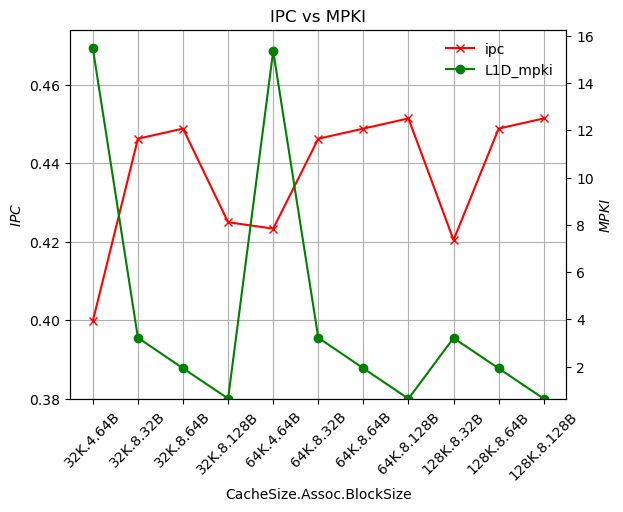
\includegraphics[width=\linewidth]{\imagesPath/L1_blackscholes.png}
					\end{center}
				\end{figure}
							
			\subsubsection{bodytrack}
				\begin{figure}[H]
					\begin{center}
						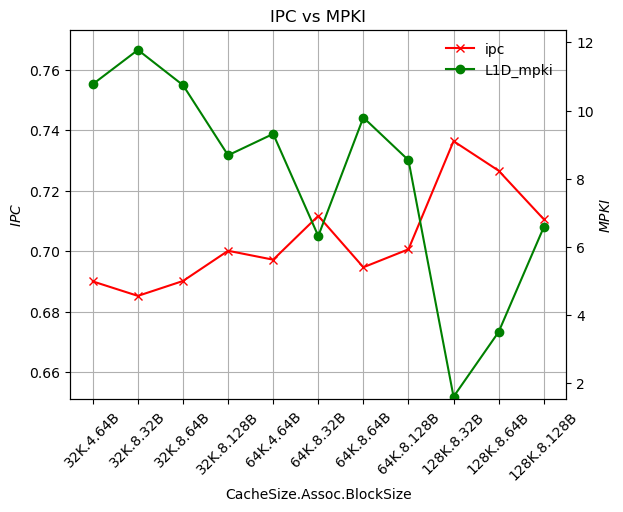
\includegraphics[width=\linewidth]{\imagesPath/L1_bodytrack.png}
					\end{center}	
				\end{figure}			
			
			\subsubsection{canneal}
				\begin{figure}[H]
					\begin{center}
						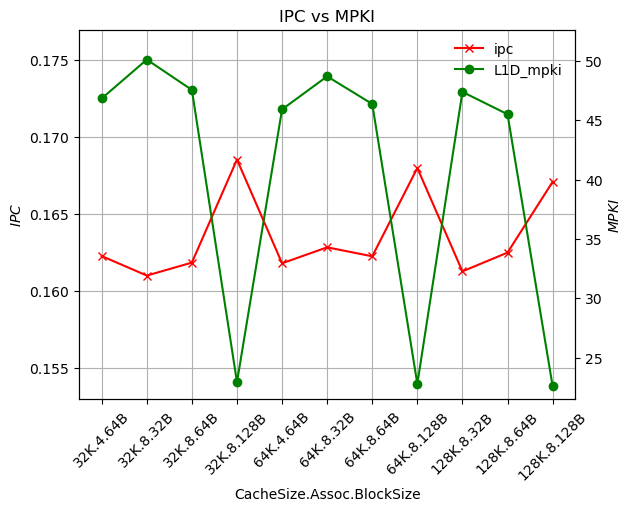
\includegraphics[width=\linewidth]{\imagesPath/L1_canneal.png}
					\end{center}
				\end{figure}
							
			\subsubsection{fluidanimate}
				\begin{figure}[H]
					\begin{center}
						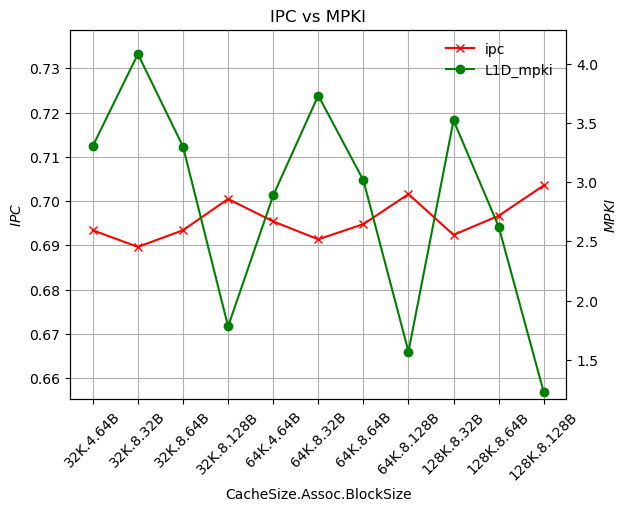
\includegraphics[width=\linewidth]{\imagesPath/L1_fluidanimate.png}
					\end{center}
				\end{figure}
						
			\subsubsection{freqmine}
				\begin{figure}[H]
					\begin{center}
						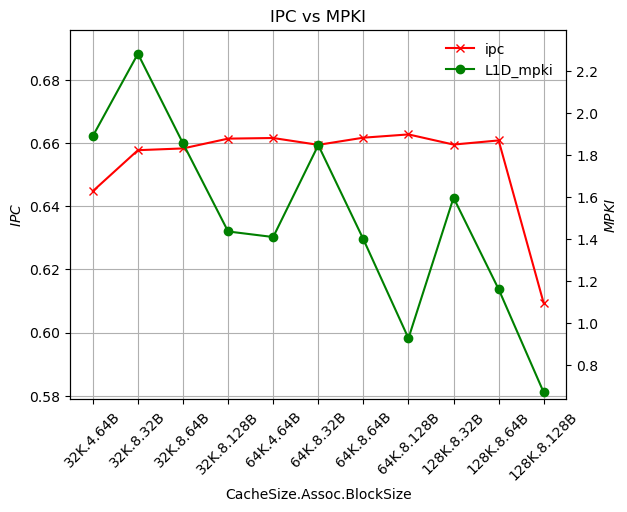
\includegraphics[width=\linewidth]{\imagesPath/L1_freqmine.png}
					\end{center}
				\end{figure}			
			
			\subsubsection{rtview}
				\begin{figure}[H]
					\begin{center}
						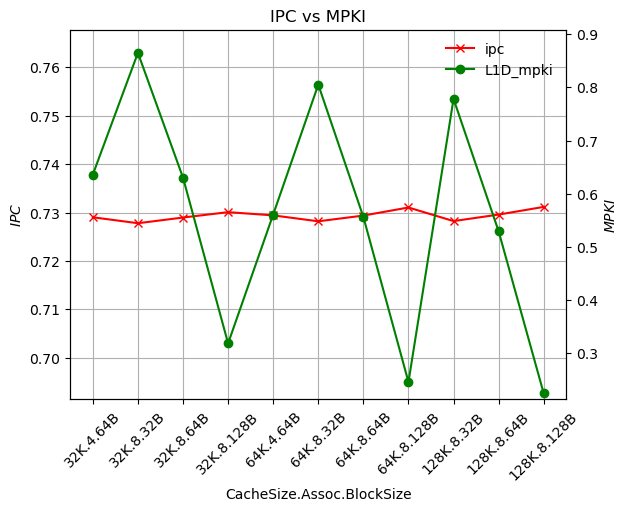
\includegraphics[width=\linewidth]{\imagesPath/L1_rtview.png}
					\end{center}
				\end{figure}
						
			\subsubsection{streamcluster}
				\begin{figure}[H]
					\begin{center}
						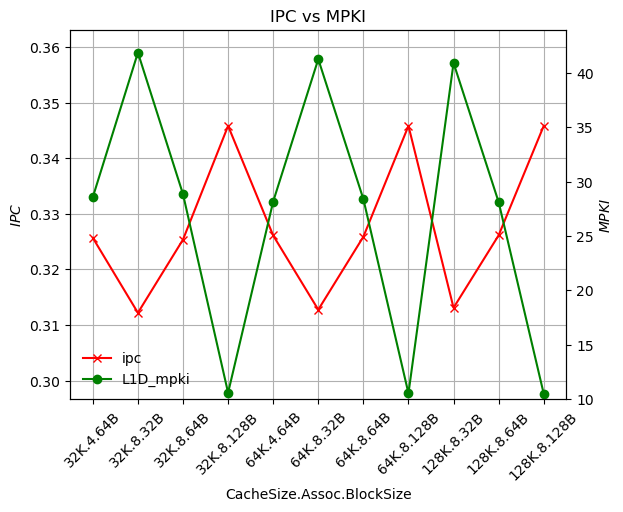
\includegraphics[width=\linewidth]{\imagesPath/L1_streamcluster.png}
					\end{center}
				\end{figure}
						
			\subsubsection{swaptions}
				\begin{figure}[H]
					\begin{center}
						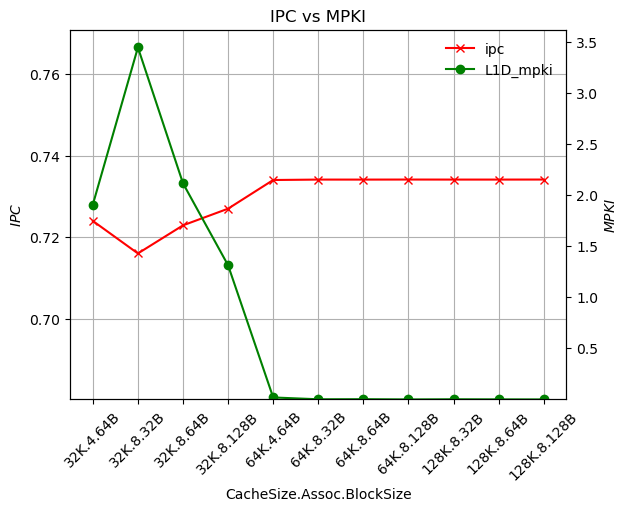
\includegraphics[width=\linewidth]{\imagesPath/L1_swaptions.png}
					\end{center}
				\end{figure}
						
			Τέλος, απεικονίζουμε το πώς μεταβάλλεται ο γεωμετρικός μέσος όρος όλων των benchmark, όσο μεταβάλλονται τα χαρακτηριστικά της cache. Ο γεωμετρικός όρος συνηθίζεται στα benchmarks, το οποίο είναι λογικό, αφού οι έννοιες του speedup και του slowdown είναι πολλαπλασιαστικής φύσεως. Για παράδειγμα, ένα speedup $\times 2$ και ένα speedup $\times 0.5$ (δηλαδή slowdown $\times 2$) έχουν γεωμετρικό μέσο ίσο με $\sqrt{2 \times 0.5} = 1$ (καθόλου συνολικό speedup), ενώ έχουν αριθμητικό μέσο $(1+0.5)/2 = 0.75$, το οποίο δεν είναι αντιπροσωπευτικό αποτέλεσμα με βάση τη διαίσθησή μας.
			
			\subsubsection{Γεωμετρικός μέσος των benchmarks}
				\begin{figure}[H]
					\begin{center}
						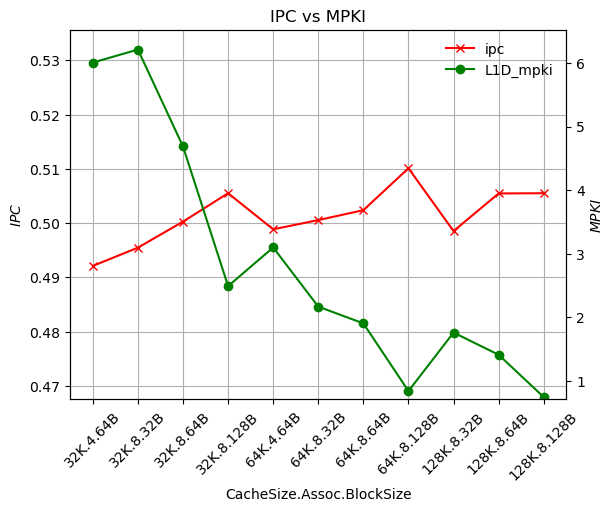
\includegraphics[width=\linewidth]{\imagesPath/L1_geoavg.png}
					\end{center}
				\end{figure}
						
			\subsubsection{Γενικές παρατηρήσεις για την L1}
				\begin{itemize}
					\item Όπως είναι λογικό τα IPC και MPKI μεταβάλλονται με αντίστροφο τρόπο (όταν το ένα αυξάνει, το άλλο μειώνεται), αφού όσο πιο πολλά misses παρατηρούνται, τόσο περισσότεροι κύκλοι απαιτούνται για να εκτελεστεί η εντολή που τα προκάλεσε.
					\item Καλύτερη επιλογή φαίνεται να είναι η τριπλέτα:
					
						\begin{verbatim}
							(cache size, associativity, block size) = (64K, 8, 128B)
						\end{verbatim} 
					\item Το L1 cache size δείχνει να βελτιώνει σημαντικά την επίδοση στο swaptions, όταν αλλάζει από 32K σε 64K.
					\item Στα benchmarks bodytrack, canneal, fluidanimate, streamcluster και swaptions παρατηρούμε ότι η αύξηση του block size μειώνει το MPKI (compulsory misses) και άρα αυξάνει το IPC (σε άλλα benchmarks περισσότερο και σε άλλα λιγότερο). 
					\item Το rtview επηρεάζεται λιγότερο σε σχέση με τα άλλα (IPC 0.70-0.71 για όλες τις τιμές των παραμέτρων).
					\item Σε όλα τα benchmarks εκτός από το swaptions, το μέγεθος της cache δεν παίζει σημαντικό ρόλο (πιθανόν να μην υπάρχουν αρκετά capacity misses ώστε το μέγεθος της cache να μπορεί να συμβάλλει).
					\item Στο blackscholes, όταν το associativity αυξήθηκε, αντίστοιχα αυξήθηκε και το IPC (άρα το πιθανότερο είναι ότι ελαττώθηκαν τα conflict misses).
					\item Τελικά οι παράμετροι που παίζουν μεγαλύτερο ρόλο είναι το associativity και το block size, και όχι τόσο το cache size.	
				\end{itemize}
			
		\subsection{L2 cache}
			Σε αυτό το κομμάτι οι παράμετροι της L1 cache και του TLB διατηρούνται σταθερές και ίσες με:

			\begin{itemize}
				\item L1 size: 32 KB
				\item L1 associativity: 8
				\item L1 block size: 64 B
				\item TLB size (entries): 64
				\item TLB associativity: 4
				\item TLB page size: 4096 B
			\end{itemize}
	
			Όσον αφορά τα χαρακτηριστικά της L2 cache, έχουμε τις εξής περιπτώσεις:
	
			\begin{center}
				\begin{tabular}{|c|c|c|}
					\hline
					L2 size (KB) & L2 associativity & L2 block size (B) \\
					\hline
					512 & 8 & 64 \\
					\hline
					512 & 8 & 128 \\
					\hline
					512 & 8 & 256 \\
					\hline
					1024 & 8 & 64 \\
					\hline
					1024 & 8 & 128 \\
					\hline
					1024 & 8 & 256 \\
					\hline
					1024 & 16 & 64 \\
					\hline
					1024 & 16 & 128 \\
					\hline
					1024 & 16 & 256 \\
					\hline
					2048 & 16 & 64 \\
					\hline 
					2048 & 16 & 128 \\
					\hline
					2048 & 16 & 256 \\
					\hline
				\end{tabular}
			\end{center}
		
			\subsubsection{blackscholes}
				\begin{figure}[H]
					\begin{center}
						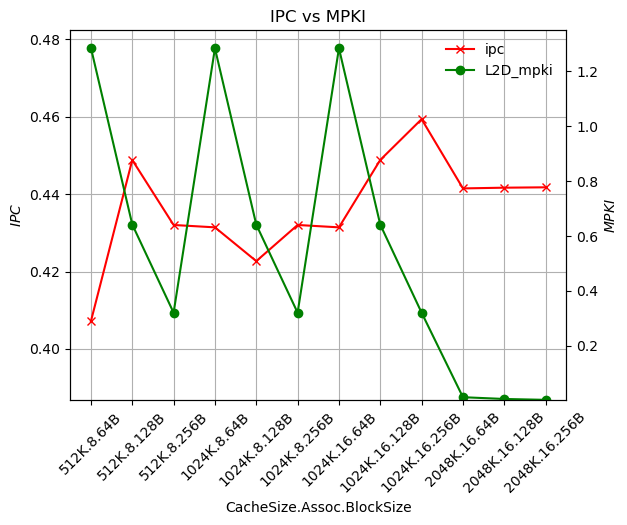
\includegraphics[width=\linewidth]{\imagesPath/L2_blackscholes.png}
					\end{center}
				\end{figure}
						
			\subsubsection{bodytrack}
				\begin{figure}[H]
					\begin{center}
						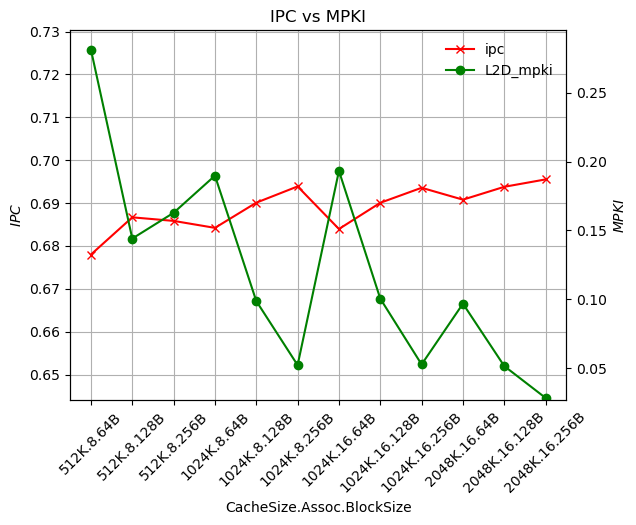
\includegraphics[width=\linewidth]{\imagesPath/L2_bodytrack.png}
					\end{center}
				\end{figure}
						
			\subsubsection{canneal}
				\begin{figure}[H]
					\begin{center}
						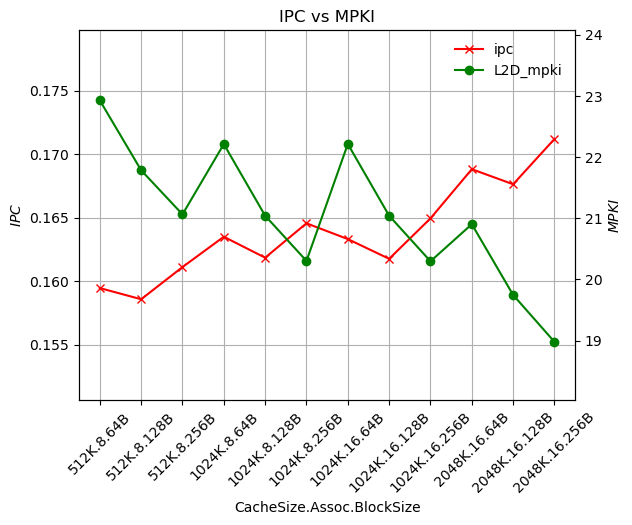
\includegraphics[width=\linewidth]{\imagesPath/L2_canneal.png}
					\end{center}
				\end{figure}
						
			\subsubsection{fluidanimate}
				\begin{figure}[H]
					\begin{center}
						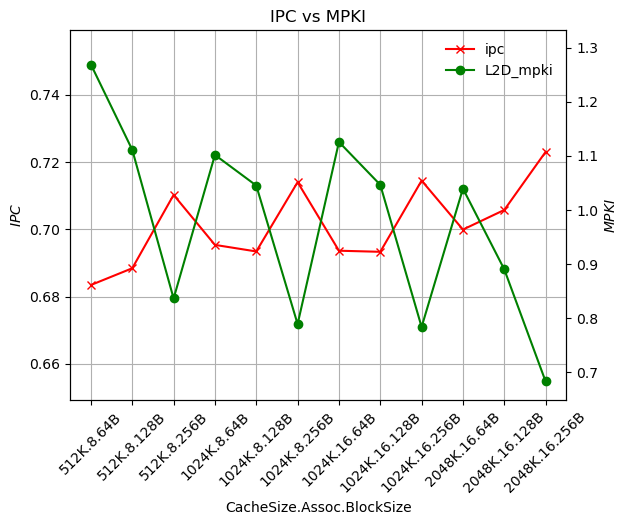
\includegraphics[width=\linewidth]{\imagesPath/L2_fluidanimate.png}
					\end{center}
				\end{figure}
						
			\subsubsection{freqmine}
				\begin{figure}[H]
					\begin{center}
						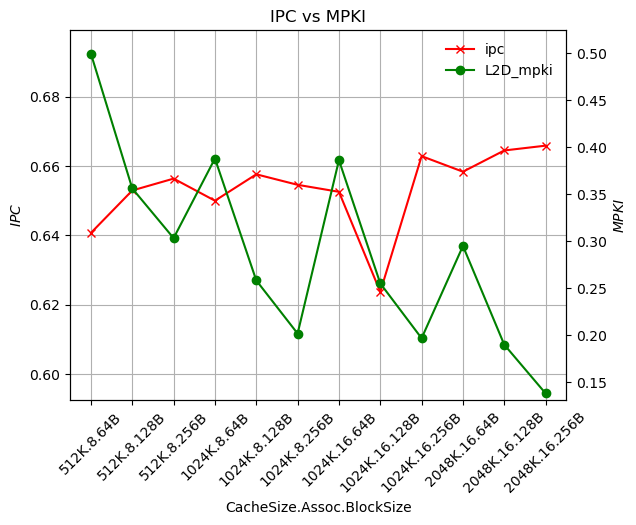
\includegraphics[width=\linewidth]{\imagesPath/L2_freqmine.png}
					\end{center}
				\end{figure}
						
			\subsubsection{rtview}
				\begin{figure}[H]
					\begin{center}
						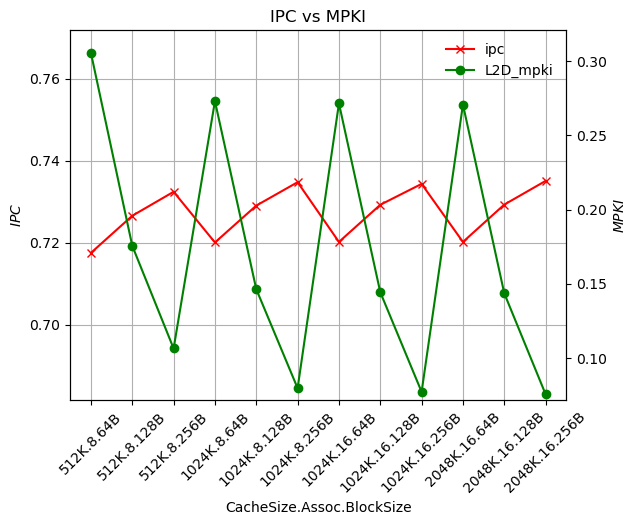
\includegraphics[width=\linewidth]{\imagesPath/L2_rtview.png}
					\end{center}
				\end{figure}
						
			\subsubsection{streamcluster}
				\begin{figure}[H]
					\begin{center}
						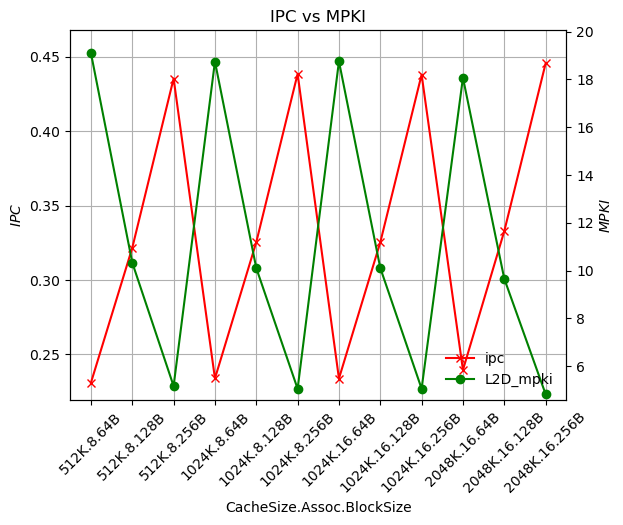
\includegraphics[width=\linewidth]{\imagesPath/L2_streamcluster.png}
					\end{center}
			
			\end{figure}
					
			\subsubsection{swaptions}
				\begin{figure}[H]
					\begin{center}
						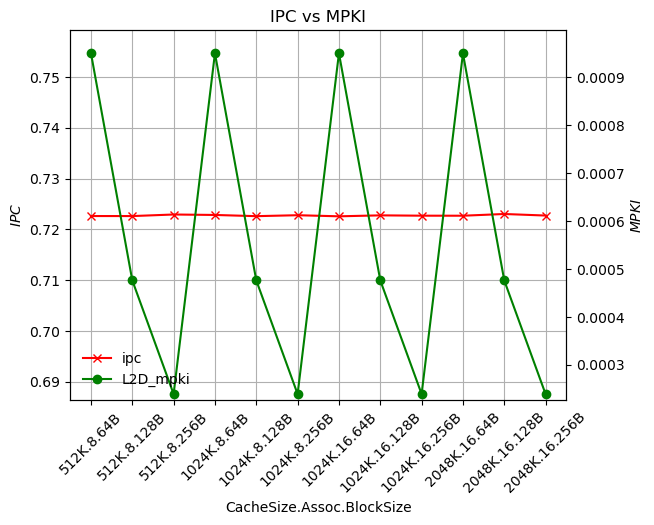
\includegraphics[width=\linewidth]{\imagesPath/L2_swaptions.png}
					\end{center}
				\end{figure}
					
			Για τους ίδιους λόγους που εξηγήθηκαν παραπάνω, παρουσιάζουμε και τον γεωμετρικό μέσο των benchmarks:
			
			\subsubsection{Γεωμετρικός μέσος των benchmarks}
				\begin{figure}[H]
					\begin{center}
						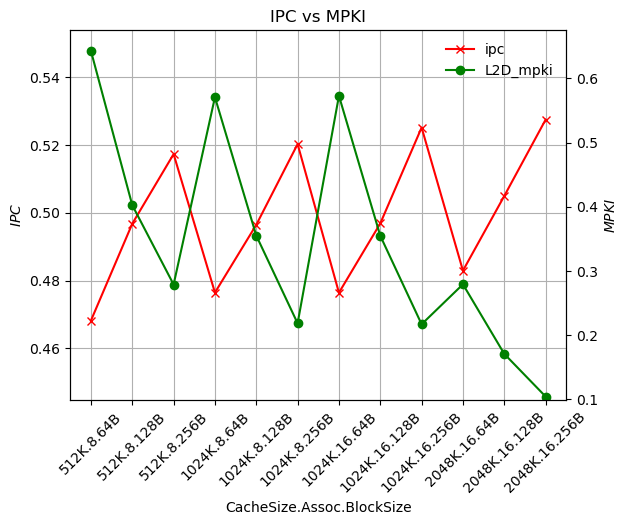
\includegraphics[width=\linewidth]{\imagesPath/L2_geoavg.png}
					\end{center}
				\end{figure}
				
			\subsubsection{Γενικές παρατηρήσεις για την L2}
				\begin{itemize}
					\item Ό,τι αναφέρθηκε παραπάνω για την αντίστροφη σχέση IPC/MPKI εξακολουθεί να ισχύει.
					\item Καλύτερη επιλογή φαίνεται να είναι η τριπλέτα:
					
						\begin{verbatim}
							(cache size, associativity, block size) = (2048K, 16, 256B)
						\end{verbatim}
					\item Η αύξηση του block size επιφέρει μείωση των compulsory misses και άρα αύξηση του IPC στα benchmarks bodytrack, fluidanimate, blackscholes, rtview, streamcluster.
					\item Στο blackscholes, φαίνεται ότι για cache size 1024K έχουμε σημαντική βελτίωση της επίδοσης, η οποία δεν μπορεί να βελτιωθεί παραπάνω με αύξηση των υπολοίπων παραμέτρων. 
					\item Στα benchmarks canneal, fluidanimate παρατηρούμε ότι όταν αυξάνουμε το μέγεθος της cache μειώνονται τα capacity misses και άρα βελτιώνεται το IPC.
					\item Το swaptions φαίνεται να μην επηρεάζεται σχεδόν καθόλου από τις αλλαγές στα χαρακτηριστικά (IPC σχεδόν σταθερό), οπότε μπορεί να χρησιμοποιούνται συνεχώς τα ίδια blocks, ή να μην χρειάζονται ξανά όσα φεύγουν από την cache.
					\item Γενικά, το block size παίζει αρκετά σημαντικό ρόλο εδώ, αν και οι άλλες δύο παράμετροι έχουν κι αυτές κάποια σημασία.
				\end{itemize}
		
		\subsection{TLB}
			Σε αυτό το κομμάτι οι παράμετροι της L1 cache και της L2 cache διατηρούνται σταθερές και ίσες με:
			
			\begin{itemize}
				\item L1 size: 32 KB
				\item L1 associativity: 8
				\item L1 block size: 64 B
				\item L2 size: 1024 KB
				\item L2 associativity: 8
				\item L2 block size: 128 B
			\end{itemize}
			
			Όσον αφορά τα χαρακτηριστικά του TLB, έχουμε τις εξής περιπτώσεις:
			
			\begin{center}
				\begin{tabular}{|c|c|c|}
					\hline
					TLB size (entries) & TLB associativity & TLB page size (B) \\
					\hline
					64 & 1 & 4096 \\
					\hline
					64 & 2 & 4096 \\
					\hline
					64 & 4 & 4096 \\
					\hline
					64 & 8 & 4096 \\
					\hline
					64 & 16 & 4096 \\
					\hline
					64 & 32 & 4096 \\
					\hline
					64 & 64 & 4096 \\
					\hline
					128 & 4 & 4096 \\
					\hline
					256 & 4 & 4096 \\
					\hline
				\end{tabular}
			\end{center}
		
			\subsubsection{blackscholes}
				\begin{figure}[H]
					\begin{center}
						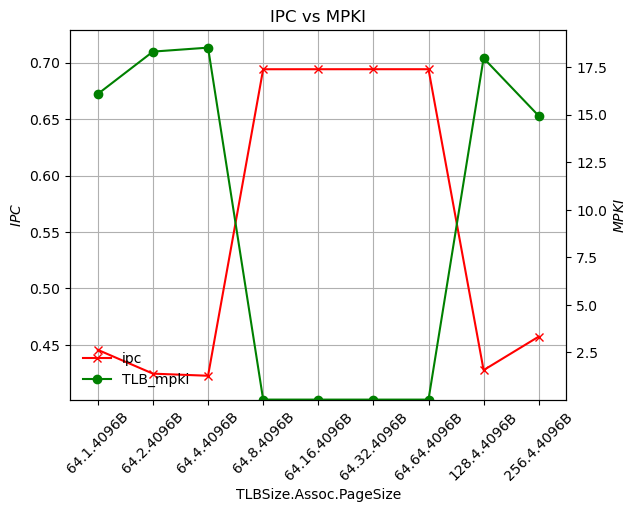
\includegraphics[width=\linewidth]{\imagesPath/TLB_blackscholes.png}
					\end{center}
				\end{figure}
						
			\subsubsection{bodytrack}
				\begin{figure}[H]
					\begin{center}
						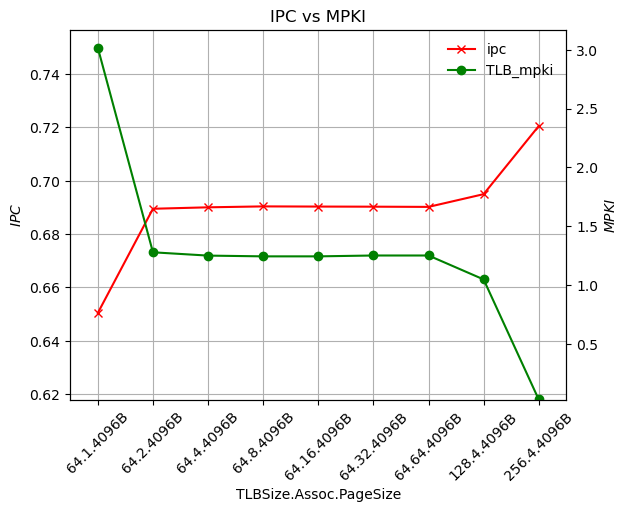
\includegraphics[width=\linewidth]{\imagesPath/TLB_bodytrack.png}
					\end{center}
				\end{figure}
						
			\subsubsection{canneal}
				\begin{figure}[H]
					\begin{center}
						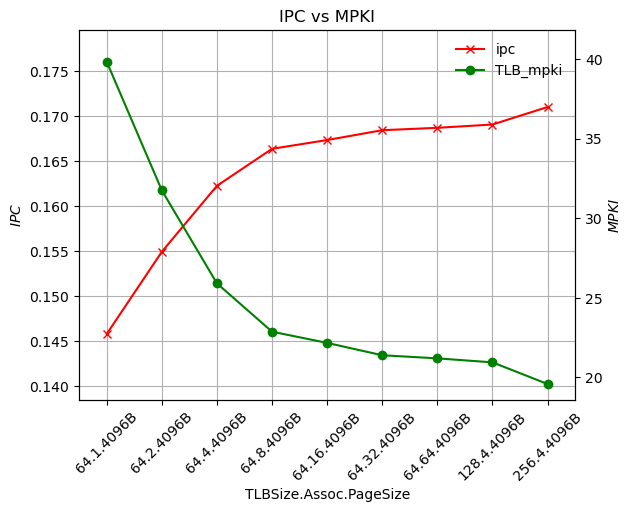
\includegraphics[width=\linewidth]{\imagesPath/TLB_canneal.png}
					\end{center}
				\end{figure}
						
			\subsubsection{fluidanimate}
				\begin{figure}[H]
					\begin{center}
						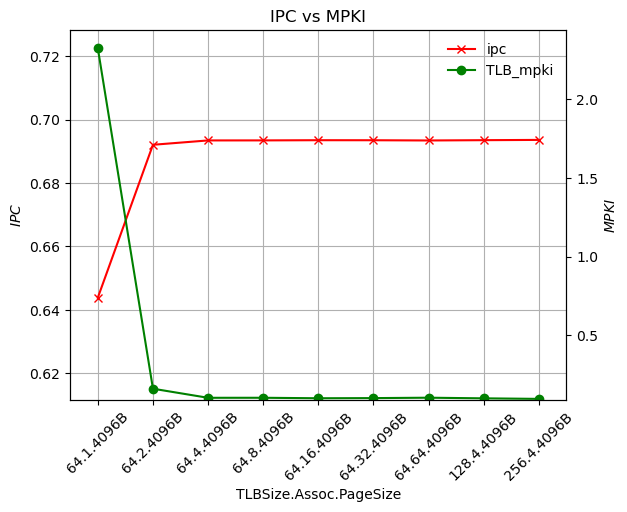
\includegraphics[width=\linewidth]{\imagesPath/TLB_fluidanimate.png}
					\end{center}
				\end{figure}
						
			\subsubsection{freqmine}
				\begin{figure}[H]
					\begin{center}
						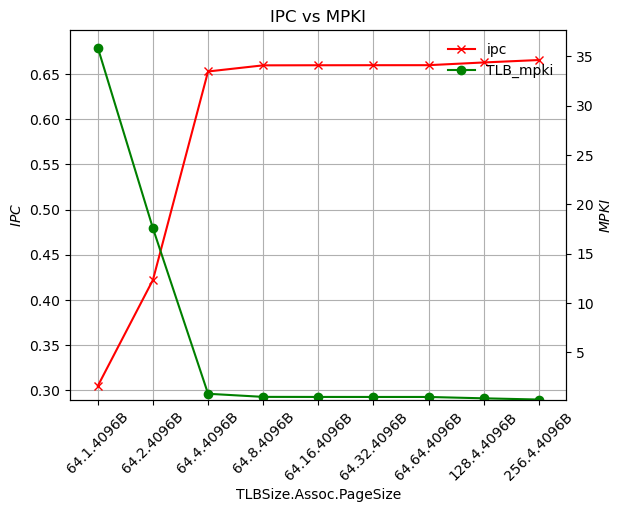
\includegraphics[width=\linewidth]{\imagesPath/TLB_freqmine.png}
					\end{center}
				\end{figure}
						
			\subsubsection{rtview}
				\begin{figure}[H]
					\begin{center}
						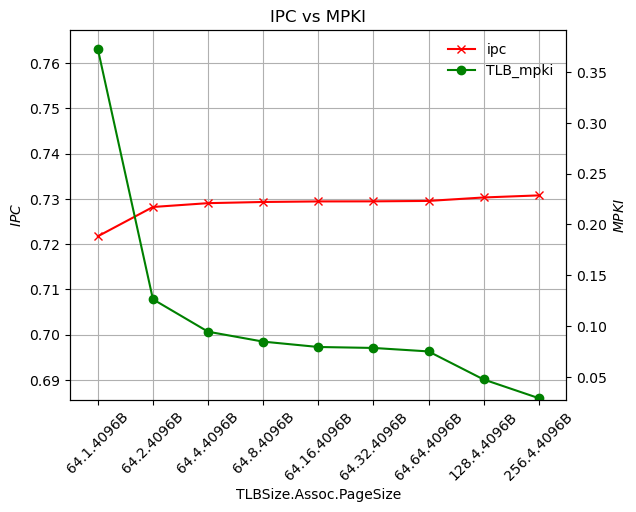
\includegraphics[width=\linewidth]{\imagesPath/TLB_rtview.png}
					\end{center}
				\end{figure}
						
			\subsubsection{streamcluster}
				\begin{figure}[H]
					\begin{center}
						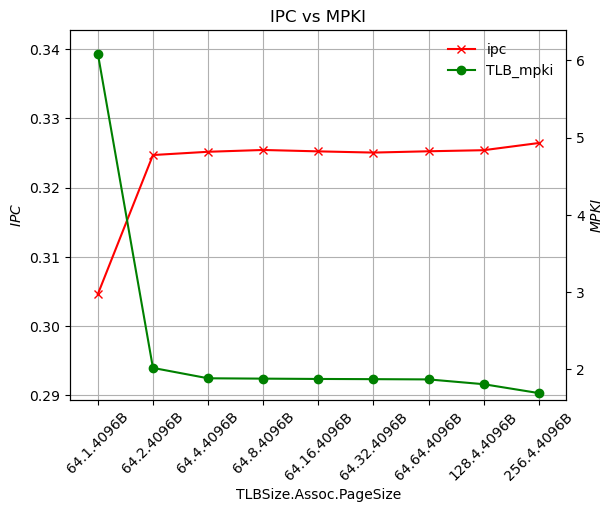
\includegraphics[width=\linewidth]{\imagesPath/TLB_streamcluster.png}
					\end{center}
				\end{figure}
						
			\subsubsection{swaptions}
				\begin{figure}[H]
					\begin{center}
						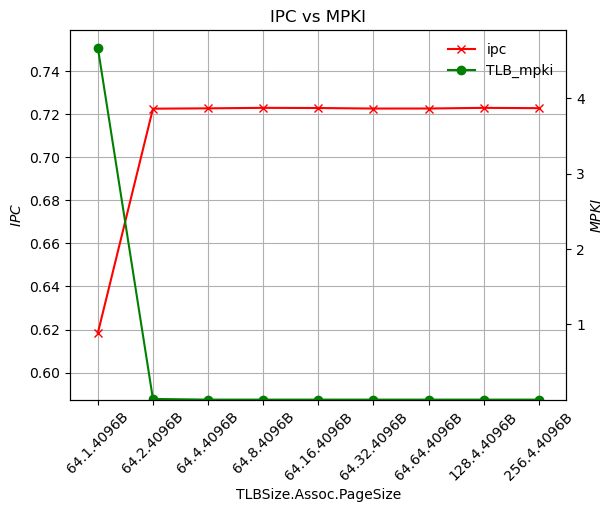
\includegraphics[width=\linewidth]{\imagesPath/TLB_swaptions.png}
					\end{center}
				\end{figure}
						
			Και εδώ δείχνουμε τον γεωμετρικό μέσο:
			
			\subsubsection{Γεωμετρικός μέσος των benchmarks}
				\begin{figure}[H]
					\begin{center}
						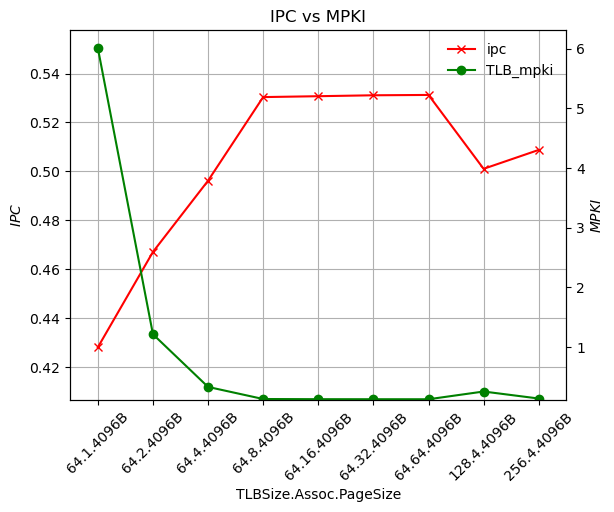
\includegraphics[width=\linewidth]{\imagesPath/TLB_geoavg.png}
					\end{center}
				\end{figure}
						
			\subsubsection{Γενικές παρατηρήσεις για το TLB}
				\begin{itemize}
					\item IPC και MPKI εξακολουθού να είναι αντιστρόφως ανάλογα.
					\item Καλύτερη επιλογή φαίνεται να είναι η τριπλέτα:
					
					\begin{verbatim}
						(TLB entries, associativity, page size) = (64, 8-64, 4096B)
					\end{verbatim}
					
					όπου το associativity δεν παίζει σχεδόν καθόλου ρόλο στην επιλογή (λογικό είναι λοιπόν να επιλέξουμε το 8, αν μεγαλύτερο associativity σημαίνει μεγαλύτερο κόστος κατασκευής).
					
					\item Όλα τα benchmarks αυτή τη φορά επηρεάστηκαν με κάποιο τρόπο από την μεταβολή των χαρακτηριστικών (σε αντίθεση με τις περιπτώσεις L1 και L2 που εξετάστηκαν παραπάνω, όπου τα rtview και swaptions αντίστοιχα έμεναν σχετικά σταθερά)
					\item Το page size δεν μπορεί να αξιολογηθεί από τα παραπάνω, αφού είναι σε όλες τις περιπτώσεις ίσο με 4096B.
					\item Η αύξηση του TLB size επιδρά πολύ λίγο στην βελτίωση του IPC.
					\item Η αύξηση του associativity φαίνεται να επιδρά πολύ θετικά στο IPC, ωστόσο κάποια στιγμή επέρχεται ένας κορεσμός (περίπου στο associativity = 8 και μετά).
				\end{itemize}
		
		\subsection{Prefetching}
			Σε αυτό το κομμάτι οι παράμετροι των L1 cache, L2 cache και TLB διατηρούνται σταθερές και ίσες με:
			
			\begin{itemize}
				\item L1 size: 32 KB
				\item L1 associativity: 8
				\item L1 block size: 64 B
				\item L2 size: 1024 KB
				\item L2 associativity: 8 
				\item L2 block size: 128 B
				\item TLB size (entries): 64 
				\item TLB associativity: 4
				\item TLB page size: 4096 B
			\end{itemize}
			
			Σε αντίθεση με τα παραπάνω, όπου το prefetching ήταν απενεργοποιημένο, θα έχουμε NEXT-N-LINE prefetching στην L2. Το N θα παίρνει τιμές \{1, 2, 4, 8, 16, 32, 64\}.
		
			\subsubsection{blackscholes}
				\begin{figure}[H]
					\begin{center}
						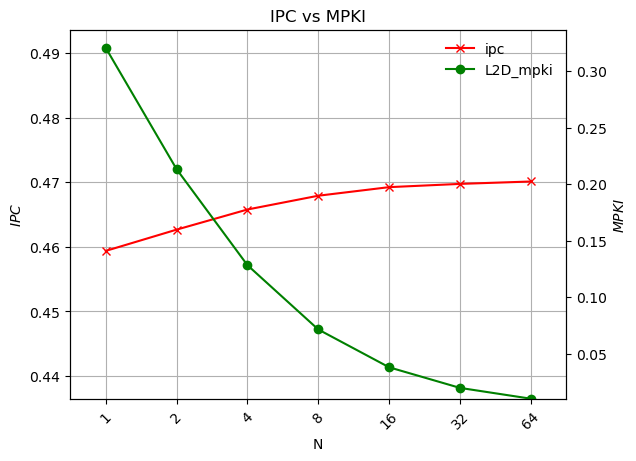
\includegraphics[width=\linewidth]{\imagesPath/PRF_blackscholes.png}
					\end{center}
				\end{figure}
			
			\subsubsection{bodytrack}
				\begin{figure}[H]
					\begin{center}
						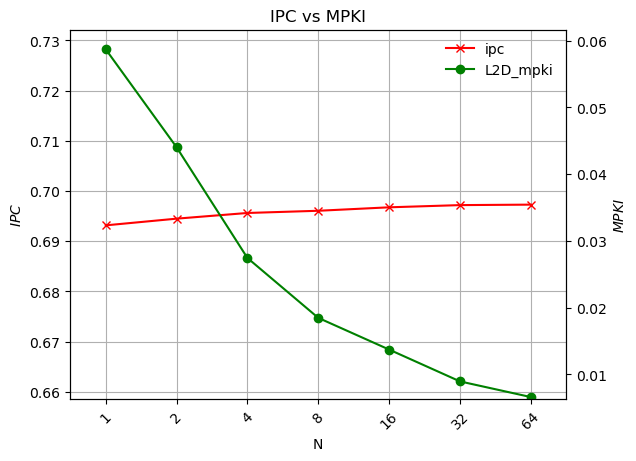
\includegraphics[width=\linewidth]{\imagesPath/PRF_bodytrack.png}
					\end{center}
				\end{figure}

			\subsubsection{canneal}
				\begin{figure}[H]
					\begin{center}
						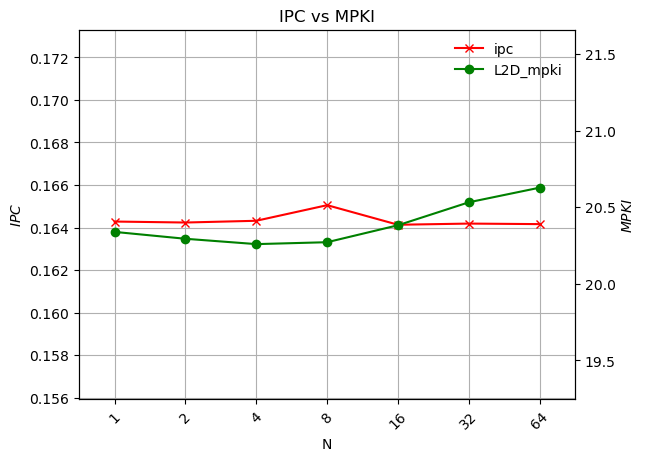
\includegraphics[width=\linewidth]{\imagesPath/PRF_canneal.png}
					\end{center}
				\end{figure}

			\subsubsection{fluidanimate}
				\begin{figure}[H]
					\begin{center}
						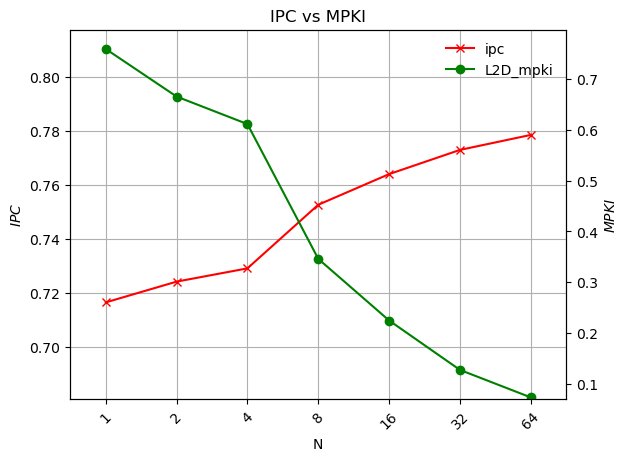
\includegraphics[width=\linewidth]{\imagesPath/PRF_fluidanimate.png}
					\end{center}
				\end{figure}
			
			\subsubsection{freqmine}
				\begin{figure}[H]
					\begin{center}
						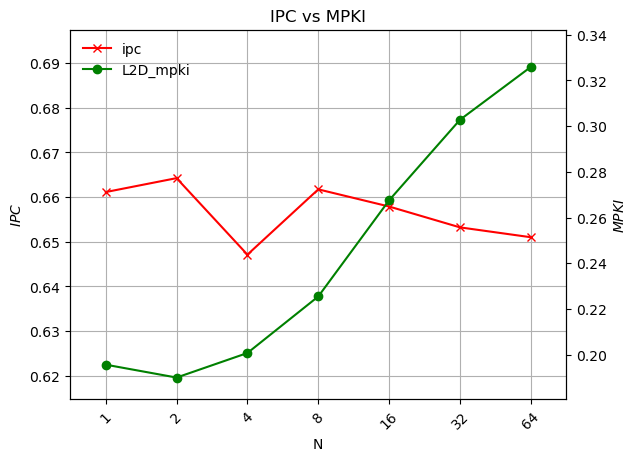
\includegraphics[width=\linewidth]{\imagesPath/PRF_freqmine.png}
					\end{center}
				\end{figure}

			\subsubsection{rtview}
				\begin{figure}[H]
					\begin{center}
						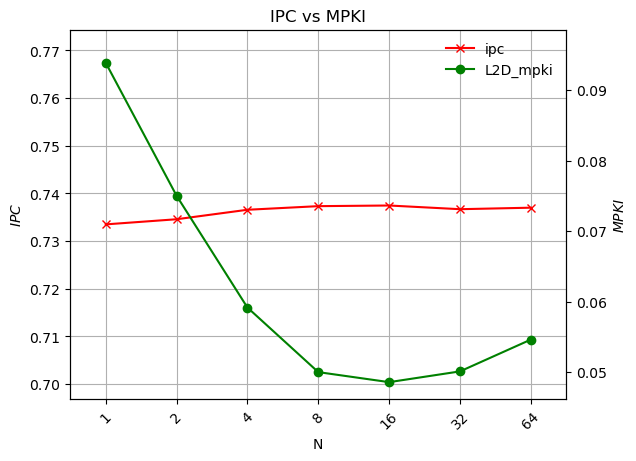
\includegraphics[width=\linewidth]{\imagesPath/PRF_rtview.png}
					\end{center}
				\end{figure}
			
			\subsubsection{streamcluster}
				\begin{figure}[H]
					\begin{center}
						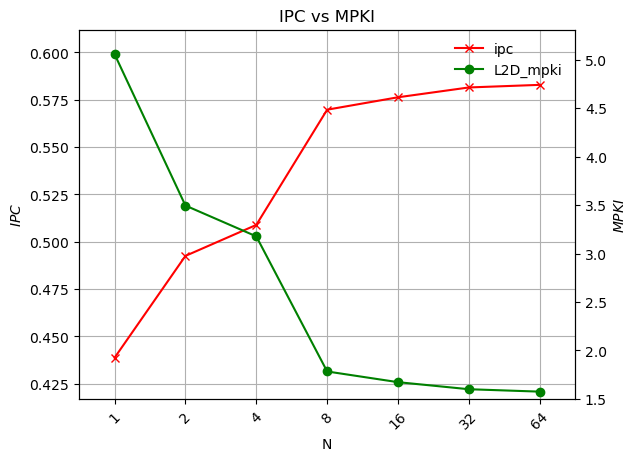
\includegraphics[width=\linewidth]{\imagesPath/PRF_streamcluster.png}
					\end{center}
				\end{figure}
			
			\subsubsection{swaptions}
				\begin{figure}[H]
					\begin{center}
						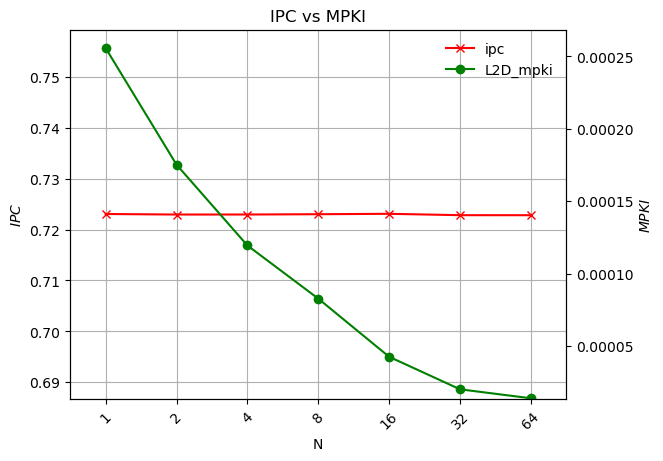
\includegraphics[width=\linewidth]{\imagesPath/PRF_swaptions.png}
					\end{center}
				\end{figure}
						
			\subsubsection{Γεωμετρικός μέσος των benchmarks}
				\begin{figure}[H]
					\begin{center}
						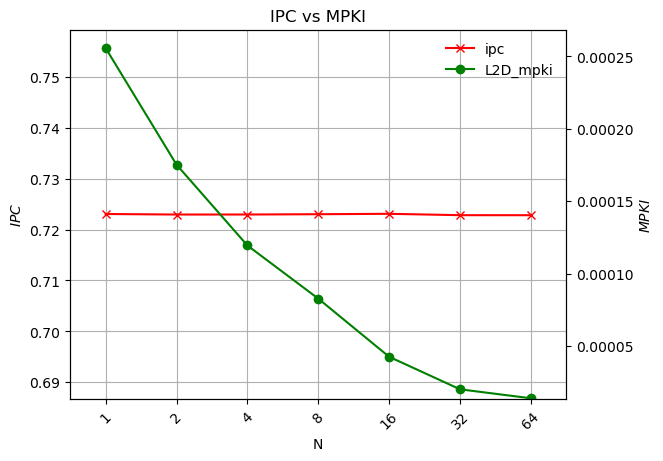
\includegraphics[width=\linewidth]{\imagesPath/PRF_geoavg.png}
					\end{center}
				\end{figure}

			\subsubsection{Γενικές παρατηρήσεις για το prefetching στην L2}
				\begin{itemize}
					\item Δεν φαίνεται να υπάρχει καθαρά καλύτερη επιλογή σε αυτή την περίπτωση (τουλάχιστον χρησιμοποιώντας σαν μετρική το IPC). Αν πραγματικά θέλουμε να διαλέξουμε την καλύτερη δυνατή επιλογή, θα χρησιμοποιήσουμε σαν μετρική το MPKI και θα επιλέξουμε N = 64, όπως είναι λογικό.
					\item Υπάρχουν αρκετά benchmarks που δεν επηρεάζονται σχεδόν καθόλου από το prefetching (bodytrack, canneal, rtview, swaptions), οπότε σε αυτά τα benchmarks μπορούμε να πούμε με σχετική σιγουριά ότι δεν γίνονται προσβάσεις σε διαχοδικά blocks.
					\item Στα υπόλοιπα benchmarks υπάρχει σχετική αύξηση (fluidanimate), ενώ στο streamcluster υπάρχει ραγδαία αύξηση όσο αυξάνεται το prefetching.
					\item Τέλος, το freqmine εμφανίζει μείωση για πιο επιθετικό prefetching, κάτι που μπορεί να οφείλεται στο ότι διώχνονται blocks που μπορεί να χρησιμοποιεί το πρόγραμμα για χάρη του prefetching.
					\item Συμπερασματικά, το prefetching είναι γενικά ωφέλιμο, μέχρι ενός ορίου.
				\end{itemize}

	\section{Ζητούμενο 2ο}
		Επειδή στην πράξη οι τροποποιήσεις στην μικροαρχιτεκτονική του επεξεργαστή προκαλούν αλλαγές στην διάρκεια του κύκλου ρολογιού, κάνουμε την υπόθεση ότι ο διπλασιασμός του associativity προκαλεί αύξηση του κύκλου κατά 10\%, ενώ ο διπλασιασμός του μεγέθους προκαλεί αύξηση 15\%. Έτσι χρησιμοποιούμε ως αναφορά την πρώτη μέτρηση που εκτελέσαμε σε κάθε benchmark και αναλόγως μεταβάλλουμε τον κύκλο ρολογιού στις επόμενες μετρήσεις. Έτσι, αν ορίσουμε:
		
		\[
			M = \dfrac{\text{Νέα τιμή associativity}}{\text{Παλιά τιμή associativity}}
		\]
		
		και:
		
		\[
			N = \dfrac{\text{Νέα τιμή cache/TLB size}}{\text{Παλιά τιμή cache/TLB size}}
		\]
		
		τότε έχουμε:
		
		\[
			\text{Νέα διάρκεια κύκλου ρολογιού} = 1.10^{\log_2 M} \times 1.15^{\log_2 N} \times \text{Παλιά διάρκεια κύκλου ρολογιού}
		\]
		
		και άρα:
		
		\[
			\text{Νέο IPC} = \dfrac{\text{Παλιό IPC}}{1.10^{\log_2 M} \times 1.15^{\log_2 N}}
		\]
		
		Τα παραπάνω αποτελέσματα ισχύουν για όλες τις τιμές των $M, N \in \{..., 2^{-3}, 2^{-2}, 2^{-1}, 1, 2, 2^2, 2^3, ...\}$, αφού:
		
		\begin{itemize}
			\item αν $M > 1 \text{ ή } N > 1$, τότε το IPC μικραίνει, όπως είναι λογικό (μεγαλώνουν τα associativity και cache size),
			\item αν $Μ < 1 \text{ ή } Ν < 1$, τότε οι λογάριθμοι παίρνουν αρνητική τιμή και το IPC μεγαλώνει (πάλι αναμενόμενο, αφού μικραίνουν τα associativity και cache size),
			\item αν $M = 1 \text{ ή } N = 1$, τότε οι λογάριθμοι είναι μηδενικοί και δεν έχουμε καμία αλλαγή.
		\end{itemize} 
	
		Με βάση την παραπάνω ανάλυση έχουμε:
		
		\subsection{L1 cache}
			\subsubsection{blackscholes (clock cycle architecture-dependent)}
				\begin{figure}[H]
					\begin{center}
						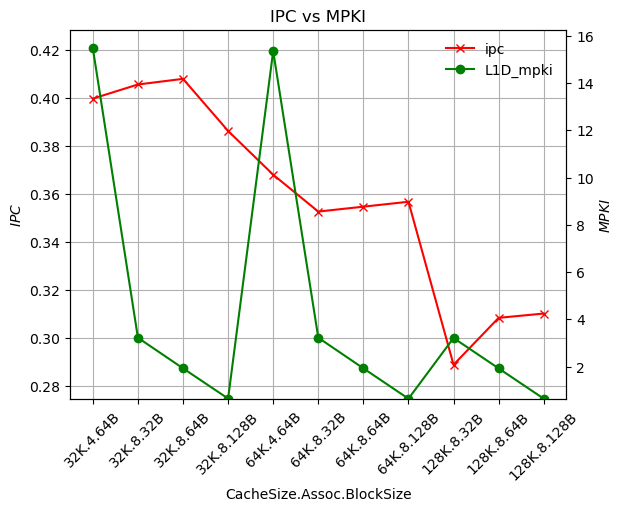
\includegraphics[width=\linewidth]{\imagesPath/L1_blackscholes_real.png}
					\end{center}
				\end{figure}
						
			\subsubsection{bodytrack (clock cycle architecture-dependent)}
				\begin{figure}[H]
					\begin{center}
						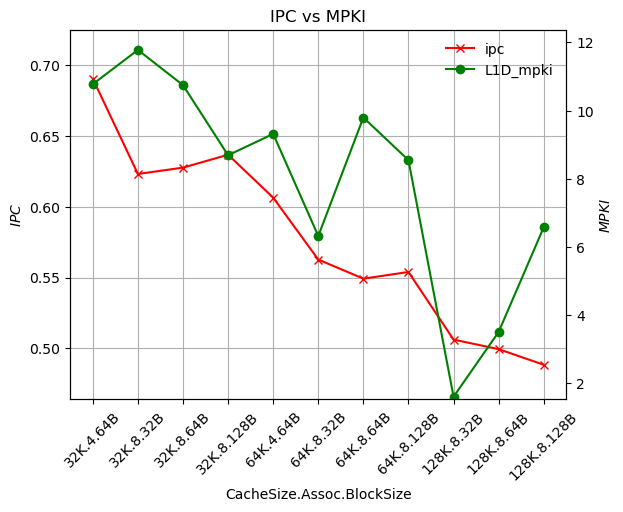
\includegraphics[width=\linewidth]{\imagesPath/L1_bodytrack_real.png}
					\end{center}
				\end{figure}
						
			\subsubsection{canneal (clock cycle architecture-dependent)}
				\begin{figure}[H]
					\begin{center}
						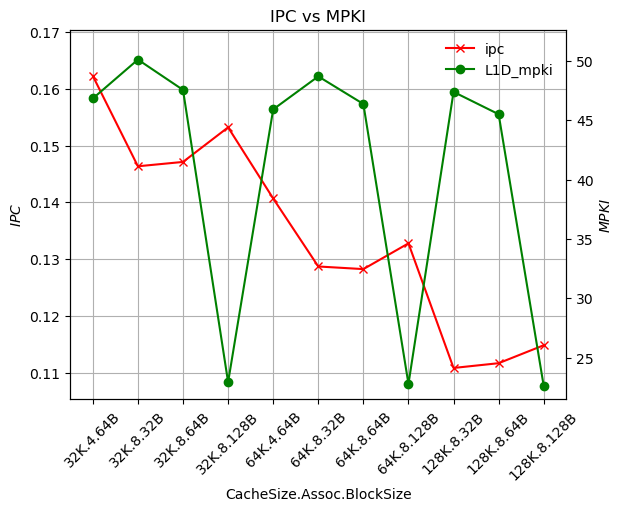
\includegraphics[width=\linewidth]{\imagesPath/L1_canneal_real.png}
					\end{center}
				\end{figure}
						
			\subsubsection{fluidanimate (clock cycle architecture-dependent)}
				\begin{figure}[H]
					\begin{center}
						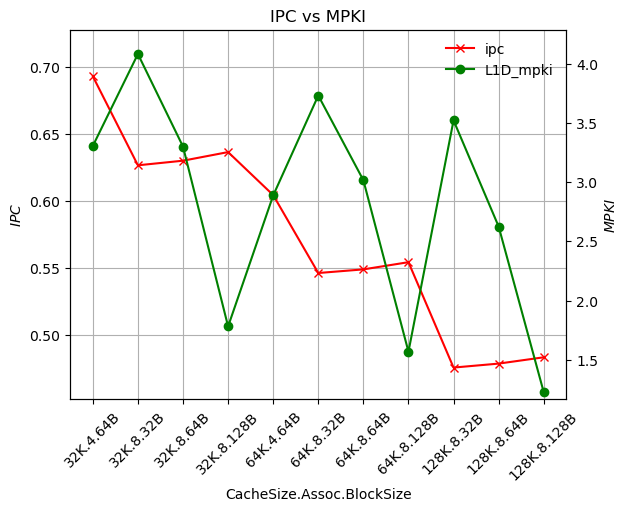
\includegraphics[width=\linewidth]{\imagesPath/L1_fluidanimate_real.png}
					\end{center}
				\end{figure}
						
			\subsubsection{freqmine (clock cycle architecture-dependent)}
				\begin{figure}[H]
					\begin{center}
						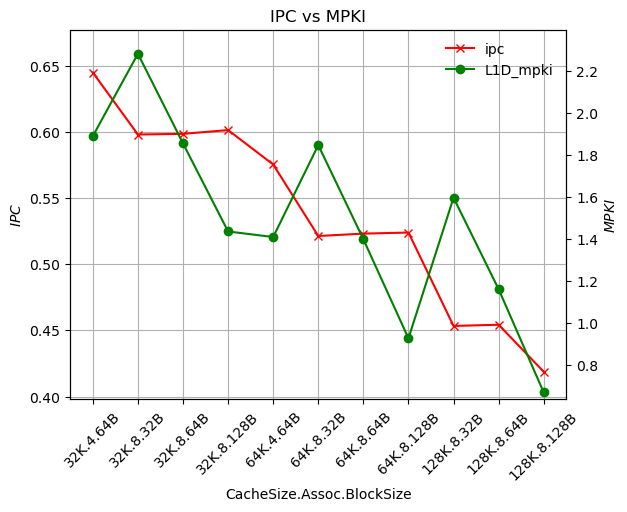
\includegraphics[width=\linewidth]{\imagesPath/L1_freqmine_real.png}
					\end{center}
				\end{figure}
						
			\subsubsection{rtview (clock cycle architecture-dependent)}
				\begin{figure}[H]
					\begin{center}
						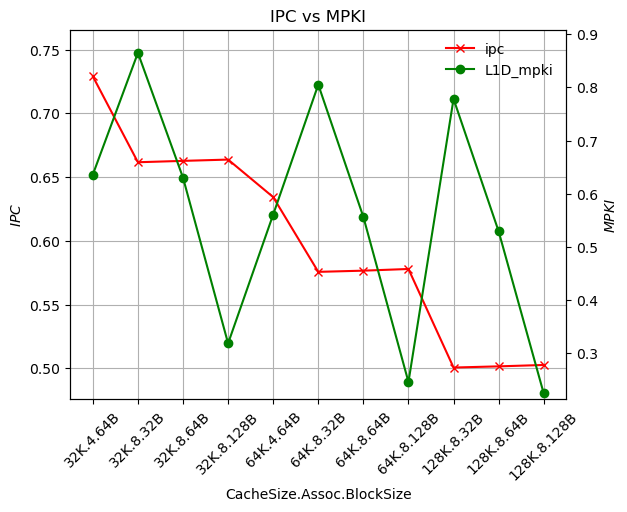
\includegraphics[width=\linewidth]{\imagesPath/L1_rtview_real.png}
					\end{center}
				\end{figure}
			
			\subsubsection{streamcluster (clock cycle architecture-dependent)}
				\begin{figure}[H]
					\begin{center}
						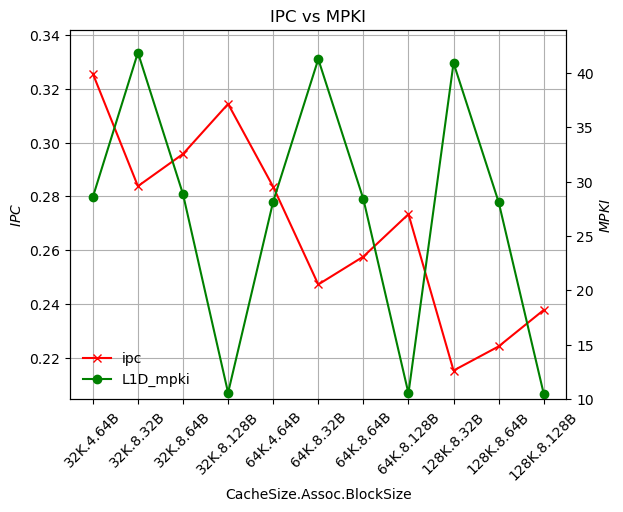
\includegraphics[width=\linewidth]{\imagesPath/L1_streamcluster_real.png}
					\end{center}
				\end{figure}
						
			\subsubsection{swaptions (clock cycle architecture-dependent)}
				\begin{figure}[H]
					\begin{center}
						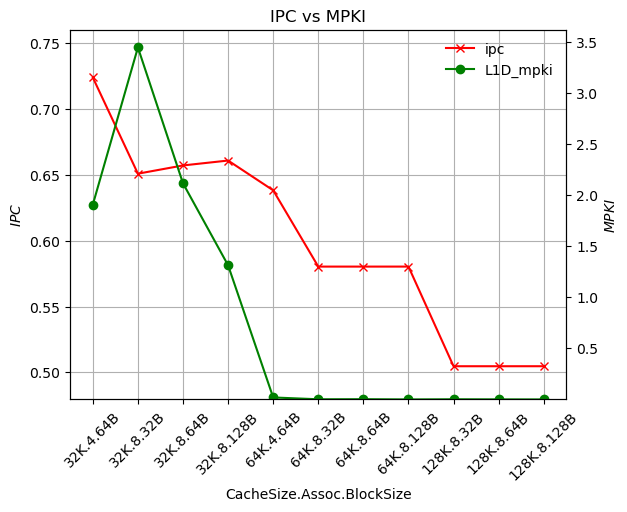
\includegraphics[width=\linewidth]{\imagesPath/L1_swaptions_real.png}
					\end{center}
				\end{figure}
						
			\subsubsection{Γεωμετρικός μέσος των benchmarks}
				\begin{figure}[H]
					\begin{center}
						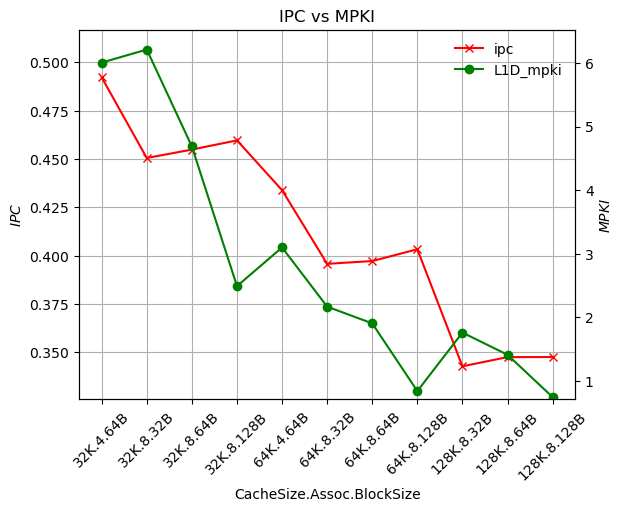
\includegraphics[width=\linewidth]{\imagesPath/L1_geoavg_real.png}
					\end{center}
			\end{figure}
				
			\subsubsection{Γενικές παρατηρήσεις για την L1 (κύκλος ρολογιού μεταβλητός)}
				\begin{itemize}
					\item Καλύτερη επιλογή φαίνεται να είναι η τριπλέτα:
						
						\begin{verbatim}
							(cache size, associativity, block size) = (32K, 4, 64B)
						\end{verbatim}
					
					\item Πλέον τα IPC και MPKI δεν είναι αντιστρόφως ανάλογα, αφού για να έχουμε λιγότερα misses πρέπει να συμβιβαστούμε με μεγαλύτερους κύκλους ρολογιού.
					\item Σε όλες τις περιπτώσεις η αύξηση των μεγεθών που δημιουργούν το επιπλέον overhead στον κύκλο ρολογιού, δηλαδή cache size και associativity, επιδρά πλέον αρνητικά στο IPC. 
					\item Το μόνο μέγεθος που είτε είναι ωφέλιμο είτε δεν επιδρά καθόλου είναι το μέγεθος του block size, αφού δεν έχει επίπτωση τον κύκλο ρολογιού.
				\end{itemize}
			
				Φαίνεται ότι όταν οι συνθήκες γίνονται πιο ρεαλιστικές (ώστε ο κύκλος ρολογιού να εξαρτάται από τα μικροαρχιτεκτονικά χαρακτηριστικά του επεξεργαστή), τα οφέλη των αυξημένων παραμέτρων (cache size, associativity, block size) "κοστίζουν" ακριβά στο IPC, και παρά την μείωση του MPKI η επίδοση χειροτερεύει.
		
		\subsection{L2 cache}
			
			\subsubsection{blackscholes (clock cycle architecture-dependent)}
				\begin{figure}[H]
					\begin{center}
						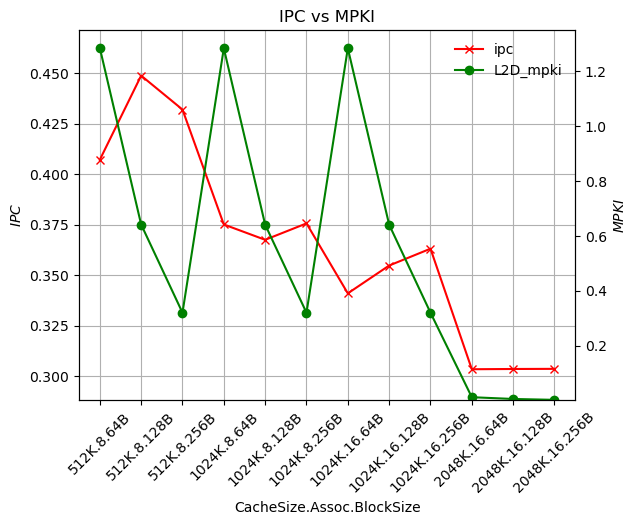
\includegraphics[width=\linewidth]{\imagesPath/L2_blackscholes_real.png}
					\end{center}
				\end{figure}
						
			\subsubsection{bodytrack (clock cycle architecture-dependent)}
				\begin{figure}[H]
					\begin{center}
						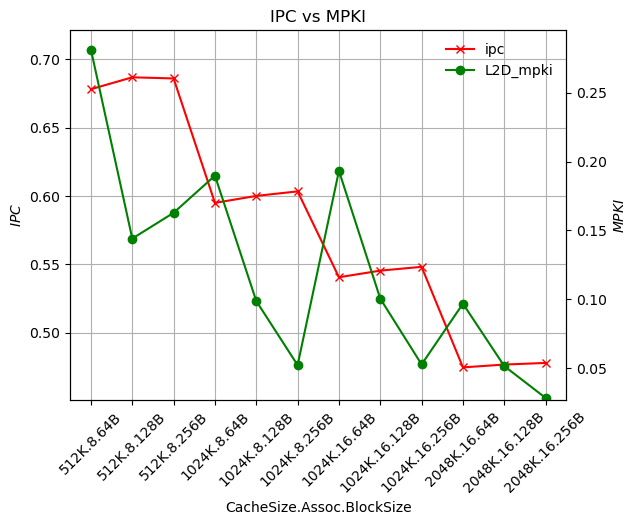
\includegraphics[width=\linewidth]{\imagesPath/L2_bodytrack_real.png}
					\end{center}
				\end{figure}
						
			\subsubsection{canneal (clock cycle architecture-dependent)}
				\begin{figure}[H]
					\begin{center}
						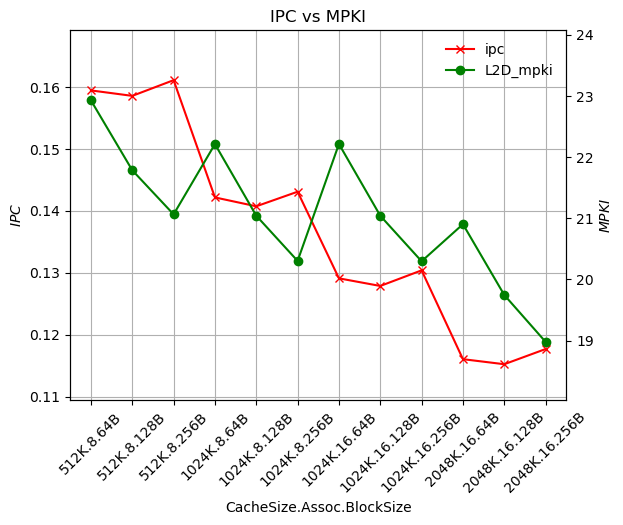
\includegraphics[width=\linewidth]{\imagesPath/L2_canneal_real.png}
					\end{center}
				\end{figure}
						
			\subsubsection{fluidanimate (clock cycle architecture-dependent)}
				\begin{figure}[H]
					\begin{center}
						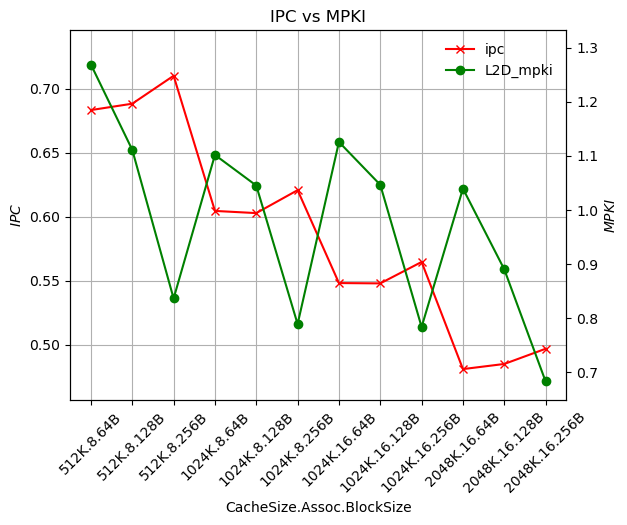
\includegraphics[width=\linewidth]{\imagesPath/L2_fluidanimate_real.png}
					\end{center}
				\end{figure}
						
			\subsubsection{freqmine (clock cycle architecture-dependent)}
				\begin{figure}[H]
					\begin{center}
						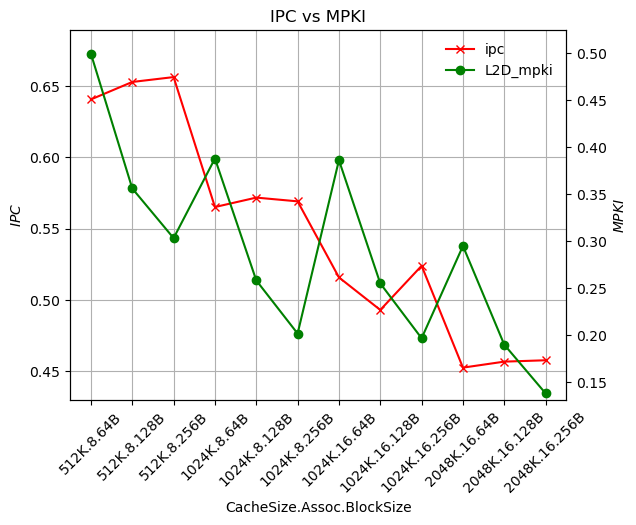
\includegraphics[width=\linewidth]{\imagesPath/L2_freqmine_real.png}
					\end{center}
				\end{figure}
						
			\subsubsection{rtview (clock cycle architecture-dependent)}
				\begin{figure}[H]
					\begin{center}
						\includegraphics[width=\linewidth]{\imagesPath/L2_rtview_real.png}
					\end{center}
				\end{figure}
						
			\subsubsection{streamcluster (clock cycle architecture-dependent)}
				\begin{figure}[H]
					\begin{center}
						\includegraphics[width=\linewidth]{\imagesPath/L2_streamcluster_real.png}
					\end{center}
				\end{figure}
						
			\subsubsection{swaptions (clock cycle architecture-dependent)}
				\begin{figure}[H]
					\begin{center}
						\includegraphics[width=\linewidth]{\imagesPath/L2_swaptions_real.png}
					\end{center}
				\end{figure}
						
			\subsubsection{Γεωμετρικός μέσος των benchmarks}
				\begin{figure}[H]
					\begin{center}
						\includegraphics[width=\linewidth]{\imagesPath/L2_geoavg_real.png}
					\end{center}
				\end{figure}
					
			\subsubsection{Γενικές παρατηρήσεις για την L2 (κύκλος ρολογιού μεταβλητός)}
				\begin{itemize}
					\item Η καλύτερη επιλογή φαίνεται να είναι η τριπλέτα:
					
						\begin{verbatim}
							(cache size, associativity, block size) = (512K, 8, 256B)
						\end{verbatim}
					\item Εδώ ισχύουν τα ίδια με την L1, απλώς εδώ η αύξηση του block size μας δίνει αρκετά μεγαλύτερο όφελος.
			\end{itemize}
		
		\subsection{TLB}
			
			\subsubsection{blackscholes (clock cycle architecture-dependent)}
				\begin{figure}[H]
					\begin{center}
						\includegraphics[width=\linewidth]{\imagesPath/TLB_blackscholes_real.png}
					\end{center}
				\end{figure}
						
			\subsubsection{bodytrack (clock cycle architecture-dependent)}
				\begin{figure}[H]
					\begin{center}
						\includegraphics[width=\linewidth]{\imagesPath/TLB_bodytrack_real.png}
					\end{center}
				\end{figure}
						
			\subsubsection{canneal (clock cycle architecture-dependent)}
				\begin{figure}[H]
					\begin{center}
						\includegraphics[width=\linewidth]{\imagesPath/TLB_canneal_real.png}
					\end{center}
				\end{figure}
						
			\subsubsection{fluidanimate (clock cycle architecture-dependent)}
				\begin{figure}[H]
					\begin{center}
						\includegraphics[width=\linewidth]{\imagesPath/TLB_fluidanimate_real.png}
					\end{center}
				\end{figure}
						
			\subsubsection{freqmine (clock cycle architecture-dependent)}
				\begin{figure}[H]
					\begin{center}
						\includegraphics[width=\linewidth]{\imagesPath/TLB_freqmine_real.png}
					\end{center}
				\end{figure}
						
			\subsubsection{rtview (clock cycle architecture-dependent)}
				\begin{figure}[H]
					\begin{center}
						\includegraphics[width=\linewidth]{\imagesPath/TLB_rtview_real.png}
					\end{center}
				\end{figure}
						
			\subsubsection{streamcluster (clock cycle architecture-dependent)}
				\begin{figure}[H]
					\begin{center}
						\includegraphics[width=\linewidth]{\imagesPath/TLB_streamcluster_real.png}
					\end{center}
				\end{figure}
						
			\subsubsection{swaptions (clock cycle architecture-dependent)}
				\begin{figure}[H]
					\begin{center}
						\includegraphics[width=\linewidth]{\imagesPath/TLB_swaptions_real.png}
					\end{center}
				\end{figure}
						
			\subsubsection{Γεωμετρικός μέσος των benchmarks}
				\begin{figure}[H]
					\begin{center}
						\includegraphics[width=\linewidth]{\imagesPath/TLB_geoavg_real.png}
					\end{center}
				\end{figure}
					
			\subsubsection{Γενικές παρατηρήσεις για το TLB (κύκλος ρολογιού μεταβλητός)}
				\begin{itemize}
					\item Καλύτερη επιλογή φαίνεται να είναι η τριπλέτα:
						
						\begin{verbatim}
							(TLB entries, associativity, page size) = (64, 1, 4096B)
						\end{verbatim}
					\item Παρατηρείται η ίδια πτωτική τάση με πριν. Ούτε το TLB size ούτε το associativity επωφελούν κάπως το IPC όταν αυξάνονται.
				\end{itemize}
\end{document}